%%%%%%%%%%%%%%%%%%%%%%%%%%%%%%%%%%%%%%%%%%%%%%%%%%%%%%%%%%%%%%%
% Gaussian Splat Capture Method Flowchart
% Paste into Overleaf to compile.
%%%%%%%%%%%%%%%%%%%%%%%%%%%%%%%%%%%%%%%%%%%%%%%%%%%%%%%%%%%%%%%
\documentclass{article}
\usepackage[margin=0.7cm, paperwidth=48cm, paperheight=21cm]{geometry}
\usepackage{graphicx}
\usepackage{tikz}
\usetikzlibrary{shapes.geometric, arrows}

% ---- Node styles ----
\tikzstyle{startstop} = [rectangle, rounded corners,
  minimum width=4cm, minimum height=1cm,
  text centered, text width=4cm,
  draw=black, fill=red!30]

\tikzstyle{subject} = [rectangle,
  minimum width=3.5cm, minimum height=1cm,
  text centered, text width=3.5cm,
  draw=black, fill=blue!15]

\tikzstyle{decision} = [diamond, aspect=2,
  text centered, text width=3cm,
  draw=black, fill=yellow!25,
  inner sep=2pt]

\tikzstyle{result} = [rectangle, rounded corners,
  minimum width=4cm, minimum height=1.2cm,
  text centered, text width=4cm,
  draw=black, fill=green!35]

\tikzstyle{arrow} = [thick,->,>=stealth]

\begin{document}

{\centering\Large\textbf{SO YOU WANT TO MAKE A GAUSSIAN SPLAT...}\par}
\vspace{0.4cm}

\noindent\resizebox{\textwidth}{!}{%
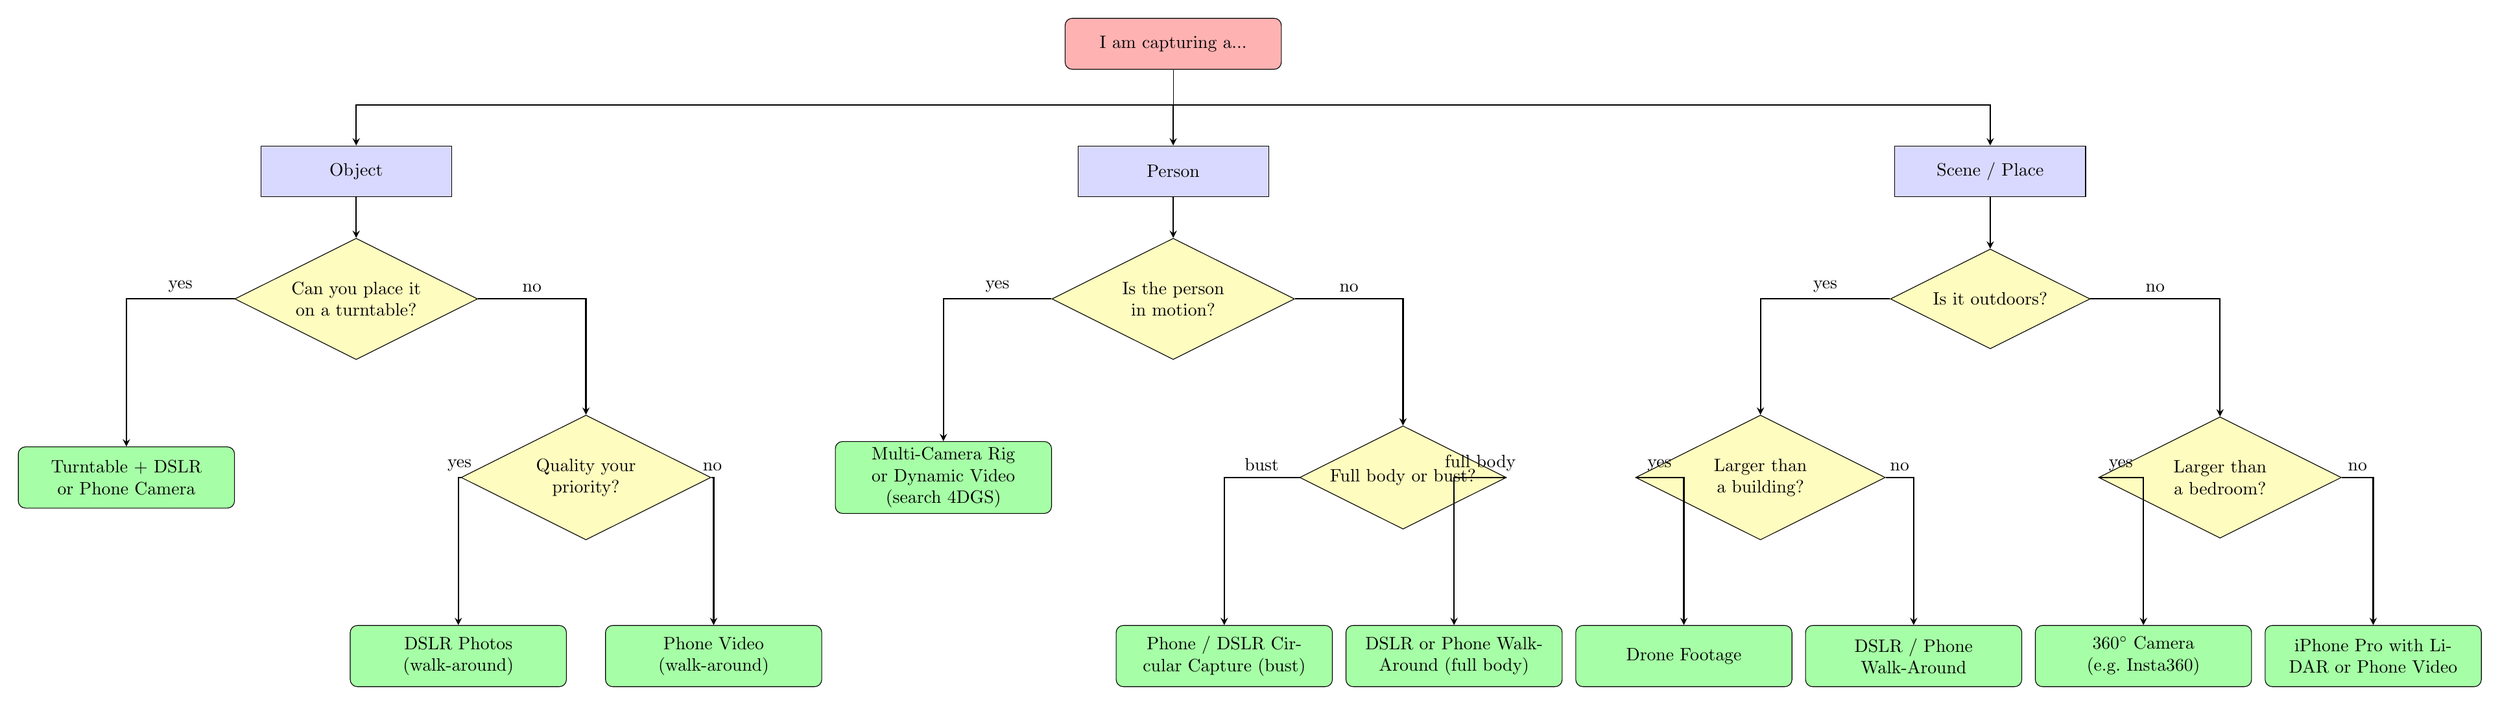
\begin{tikzpicture}

%% ---- ROOT ----
\node (root) [startstop] at (0, 0) {I am capturing a...};
\coordinate (split) at (0, -1.2);
\draw (root.south) -- (split);

%% ---- SUBJECT BRANCHES ----
\node (obj) [subject] at (-16, -2.5) {Object};
\node (per) [subject] at (0,   -2.5) {Person};
\node (sce) [subject] at (16,  -2.5) {Scene / Place};

\draw[arrow] (split) -| (obj.north);
\draw[arrow] (split) -- (per.north);
\draw[arrow] (split) -| (sce.north);

%%=============================================================
%% OBJECT BRANCH
%%  Decision 1: Can you place it on a turntable?
%%    yes -> Turntable + DSLR or Phone
%%    no  -> Decision 2: Quality your priority?
%%             yes -> DSLR Photos (walk-around)
%%             no  -> Phone Video (walk-around)
%%=============================================================
\node (oq1) [decision] at (-16, -5)
  {Can you place it on a turntable?};

\node (res_tt)    [result] at (-20.5, -8.5)
  {Turntable + DSLR or Phone Camera};

\node (oq2) [decision] at (-11.5, -8.5)
  {Quality your priority?};

\node (res_dslro) [result] at (-14, -12)
  {DSLR Photos (walk-around)};

\node (res_phono) [result] at (-9,  -12)
  {Phone Video (walk-around)};

\draw[arrow] (obj)       -- (oq1);
\draw[arrow] (oq1.west)  -| node[near start, above]{yes} (res_tt);
\draw[arrow] (oq1.east)  -| node[near start, above]{no}  (oq2);
\draw[arrow] (oq2.west)  -| node[near start, above]{yes} (res_dslro);
\draw[arrow] (oq2.east)  -| node[near start, above]{no}  (res_phono);

%%=============================================================
%% PERSON BRANCH
%%  Decision 1: Is the person in motion?
%%    yes -> Multi-Camera Rig or Dynamic Video
%%    no  -> Decision 2: Full body or bust?
%%             bust      -> Phone/DSLR Circular Capture
%%             full body -> DSLR or Phone Walk-Around
%%=============================================================
\node (pq1) [decision] at (0, -5)
  {Is the person in motion?};

\node (res_mc) [result] at (-4.5, -8.5)
  {Multi-Camera Rig or Dynamic Video (search 4DGS)};

\node (pq2) [decision] at (4.5, -8.5)
  {Full body or bust?};

\node (res_bust) [result] at (1, -12)
  {Phone / DSLR Circular Capture (bust)};

\node (res_full) [result] at (5.5, -12)
  {DSLR or Phone Walk-Around (full body)};

\draw[arrow] (per)       -- (pq1);
\draw[arrow] (pq1.west)  -| node[near start, above]{yes}       (res_mc);
\draw[arrow] (pq1.east)  -| node[near start, above]{no}        (pq2);
\draw[arrow] (pq2.west)  -| node[near start, above]{bust}      (res_bust);
\draw[arrow] (pq2.east)  -| node[near start, above]{full body} (res_full);

%%=============================================================
%% SCENE BRANCH
%%  Decision 1: Is it outdoors?
%%    yes -> Decision 2: Larger than a building?
%%             yes -> Drone Footage
%%             no  -> DSLR / Phone Walk-Around
%%    no  -> Decision 2: Larger than a bedroom?
%%             yes -> 360 degree Camera
%%             no  -> iPhone Pro with LiDAR or Phone Video
%%=============================================================
\node (sq1) [decision] at (16, -5)
  {Is it outdoors?};

\node (sq2) [decision] at (11.5, -8.5)
  {Larger than a building?};

\node (res_drone) [result] at (10,  -12)
  {Drone Footage};

\node (res_walko) [result] at (14.5, -12)
  {DSLR / Phone Walk-Around};

\node (sq3) [decision] at (20.5, -8.5)
  {Larger than a bedroom?};

\node (res_360)   [result] at (19, -12)
  {$360^\circ$ Camera (e.g.\ Insta360)};

\node (res_lidar) [result] at (23.5, -12)
  {iPhone Pro with LiDAR or Phone Video};

\draw[arrow] (sce)       -- (sq1);
\draw[arrow] (sq1.west)  -| node[near start, above]{yes} (sq2);
\draw[arrow] (sq1.east)  -| node[near start, above]{no}  (sq3);
\draw[arrow] (sq2.west)  -| node[near start, above]{yes} (res_drone);
\draw[arrow] (sq2.east)  -| node[near start, above]{no}  (res_walko);
\draw[arrow] (sq3.west)  -| node[near start, above]{yes} (res_360);
\draw[arrow] (sq3.east)  -| node[near start, above]{no}  (res_lidar);

\end{tikzpicture}%
}
\end{document}
